\documentclass[conference]{IEEEtran}
\usepackage[T1]{fontenc}
\usepackage[utf8]{inputenc}
\usepackage{graphicx}
\usepackage{amsmath}
\usepackage{booktabs}
\usepackage{hyperref}
\usepackage{cite}

\begin{document}

\title{KulTur: A Chatbot That Recommends Cultural Heritage Sites in Bosnia and Herzegovina}

\author{
\IEEEauthorblockN{Džana Kopić}
\IEEEauthorblockA{Machine Learning Supervised Techniques (MLST)\\
University of Sarajevo \\
Faculty of Electrical Engineering\\
dkopic2@etf.unsa.ba}
}

\maketitle

\begin{abstract}
Bosnia and Herzegovina contains a large number of historical and cultural sites, yet most of them, especially the smaller and less well-known ones, have little to no online presence. As a result, tourists tend to visit the same small set of well-known destinations, while many other sites remain effectively invisible. This project addresses that problem by building KulTur, a chatbot that recommends heritage sites based on a user's stated interests, location, season, and available time. The system works in three stages: it first searches a database of heritage sites for entries that match the topic of the user's question, then re-ranks those results using a supervised machine learning model trained on the user's preferences, and finally uses a language model to produce a natural-sounding answer using only the retrieved information. The dataset (273 sites after cleaning) was compiled and verified manually and published openly on Kaggle. A Random Forest classifier was trained to perform the re-ranking step and was evaluated honestly on unseen data, reaching approximately 75\% accuracy; the reasoning behind preferring this figure over an initial, misleading 86\% figure is explained in detail. This report also discusses the most demanding part of the project, which was constructing and cleaning the dataset, rather than the modeling itself.
\end{abstract}

\begin{IEEEkeywords}
chatbot, random forest, retrieval, cultural heritage, tourism, Bosnia and Herzegovina
\end{IEEEkeywords}

\section{Introduction}

Bosnia and Herzegovina holds a large amount of history within a relatively small area: old fortresses, Ottoman-era buildings, Austro-Hungarian architecture, religious sites, and natural landmarks such as waterfalls and caves. In practice, however, most visitors only see a small number of well-known places, such as Mostar or Ba\v{s}\v{c}ar\v{s}ija in Sarajevo, while hundreds of smaller sites remain largely undocumented online. If a visitor does not already know that a site exists, ordinary search engines and travel applications provide little help in discovering it.

This topic was chosen out of a genuine interest in tourism and in the cultural heritage of the country, combined with an interest in applying the methods covered in this course to a real, personally meaningful problem. The idea behind KulTur is to sit between two extremes: a fully open-ended chatbot, which may produce incorrect or invented information, and a plain search filter, which is accurate but not conversational. KulTur is designed to remain conversational while being restricted to information from a dataset that was compiled and manually verified as part of this project.

\subsection{Project Goals}
Given a user's message (for example, ``I want to see some old fortresses near Travnik in autumn''), the system is expected to:
\begin{itemize}
\item identify sites that genuinely match the topic of the request,
\item rank those sites according to the user's stated preferences rather than by popularity alone,
\item and produce a reply that does not include facts, distances, or sites that are not present in the underlying dataset.
\end{itemize}

The project was guided by three main questions:
\begin{itemize}
\item Does adding a supervised ranking model on top of basic search meaningfully improve the quality of recommendations?
\item Can a chatbot remain conversational while being strictly limited to verified information?
\item How should a recommendation model be trained when no real user interaction data is available yet?
\end{itemize}

\subsection{Summary of the Approach}
Three components were combined to build the system: a search step that identifies heritage sites matching the topic of a question, using text embeddings and a vector database (ChromaDB); a Random Forest classifier that re-ranks the search results according to the user's stated preferences; and a language model that generates the final reply using only the results produced by the first two steps. A smaller location-based filter, based on a clustering method called DBSCAN, was also incorporated to keep recommendations geographically relevant; this component was originally developed for a separate course and was reused and integrated here rather than built specifically for this project, and is therefore discussed only briefly.

\subsection{Summary of Contributions}
\begin{itemize}
\item A dataset of 273 heritage sites in Bosnia and Herzegovina, compiled and manually verified from public and institutional sources, and published openly on Kaggle~\cite{kaggle}; this was the most time-consuming part of the project.
\item A two-stage recommendation pipeline combining semantic search and supervised re-ranking.
\item A Random Forest model evaluated honestly on unseen data (approximately 75\% accuracy), including an explicit discussion of why this figure, rather than a higher but misleading one, is reported as the main result.
\item A working prototype application built with Streamlit, demonstrating the complete pipeline, with source code available on GitHub~\cite{github}.
\end{itemize}

\section{Related Work}
Most existing tourism recommendation systems, including those used by large commercial travel platforms, rely on prior user behavior: what similar users liked, rated, or booked before. This approach performs well when a large amount of user history is available, but it does not work for a domain such as this one, where most of the smaller heritage sites have no existing user data at all. This situation is commonly referred to as a cold-start problem in recommendation systems, since there is no historical signal to learn from.

Separately, there has been considerable recent work on combining search with language models, commonly known as retrieval-augmented generation~\cite{rag}. Rather than allowing a language model to answer purely from what it has learned during training, the model is first given a set of retrieved, trustworthy documents and instructed to answer only using that material. This approach is often used in domains where factual accuracy is critical, such as legal or institutional question answering. KulTur applies the same general idea to tourism recommendations, while additionally introducing a supervised ranking model to personalize results, which is a less common combination than retrieval alone or collaborative filtering alone.

\section{Building the Dataset}
Of all the stages of this project, constructing the dataset required the most time and effort, considerably more than the modeling work described later in this report. Since a recommendation system can only be as reliable as the data behind it, particular care was taken during this stage rather than treating it as a preliminary step.

\subsection{Data Sourcing}
The dataset was compiled manually rather than obtained from an existing, ready-made source. Site information was gathered from a combination of institutional and public references, including the Federal Institute for Statistics~\cite{fzs}, the Commission to Preserve National Monuments~\cite{kons}, the UNESCO World Heritage list~\cite{unesco}, the Spomenik Database~\cite{spomenik}, and general public sources such as Wikipedia. Coordinates were cross-checked against these sources rather than accepted without verification. Descriptions and short factual notes for each site were partly written directly and partly drafted with AI assistance, after which each entry was manually checked against its original source before being included, rather than accepted without review. This verification process alone accounted for a significant portion of the total time spent on the project. The finished dataset was published publicly on Kaggle~\cite{kaggle} as the ``Bosnia and Herzegovina Heritage Landmarks Dataset.''

\subsection{Removing Duplicate Entries}
The initial dataset contained 300 rows and was reduced to 273 after cleaning, meaning 27 rows were removed. Almost none of this reduction was due to missing information; the primary issue was duplication, addressed in three steps:
\begin{itemize}
\item A small number of entries (3, matching 4 raw rows once spelling variants were accounted for) were removed after being manually identified as invalid or irrelevant.
\item Entries sharing identical coordinates with another entry already present in the dataset were removed, typically because the same physical location had been entered under two different names, such as ``Kravice Waterfall'' and the correctly spelled ``Kravica Waterfall.''
\item Entries with an identical name appearing more than once (for example, ``Te\v{s}anj Fortress,'' which appeared three times) were reduced to a single entry, covering 19 such groups and removing 20 rows in total.
\end{itemize}
This indicates that the main issue with the raw data was repetition rather than missing values, which required a deduplication-based cleaning approach rather than the imputation methods typically discussed for handling missing data.

\subsection{Standardizing Categories}
The initial dataset contained 49 distinct category labels, a result of inconsistent labeling introduced during manual data entry (for example, ``archeological site,'' ``historic site,'' and ``historical site'' were recorded as separate values despite referring to the same concept). This was corrected in two steps: first, a manual mapping grouped clear synonyms together (all fortress-related labels were merged into ``fortress''; fourteen nature-related labels were merged into ``nature''); second, any category still containing fewer than five sites after this step was automatically folded into either ``nature'' or a general category named ``other heritage/leisure.'' The final set consists of nine categories: archaeological, fortress, monument, museum, nature, other heritage/leisure, religious, traditional village, and urban heritage.

\subsection{Dataset Fields}
Each of the 273 entries contains 22 fields, including name, description, keywords, region (seven possible values: Central Bosnia, Eastern Bosnia, Herzegovina, Krajina, Northern Bosnia, Sarajevo Region, or ``Any''), historical period (36 specific values, grouped into six broader categories: Ancient, Medieval, Modern, Multi-Era, Other, Ottoman), category, coordinates, a popularity level, applicable tourist seasons, and average visit duration. The last of these required a dedicated parsing function to convert text such as ``2--3 hours'' into a numeric value suitable for modeling.

A recurring technical difficulty throughout this stage was the presence of Bosnian-language characters (\'{c}, \v{c}, \v{s}, \dj, \v{z}) in nearly every site name, which repeatedly caused character-encoding errors during processing on Windows and required explicit UTF-8 handling to be applied consistently throughout the codebase.

\begin{figure}[htbp]
\centering
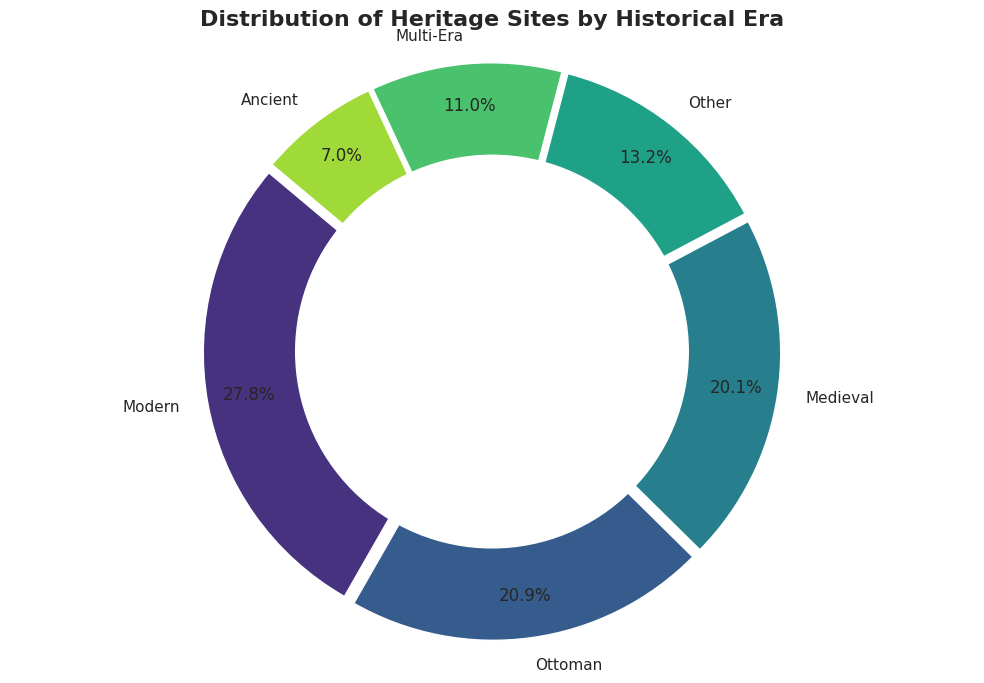
\includegraphics[width=\linewidth]{figures/era_donut.png}
\caption{Distribution of the 273 heritage sites by historical era.}
\label{fig:era_donut}
\end{figure}

\begin{figure}[htbp]
\centering
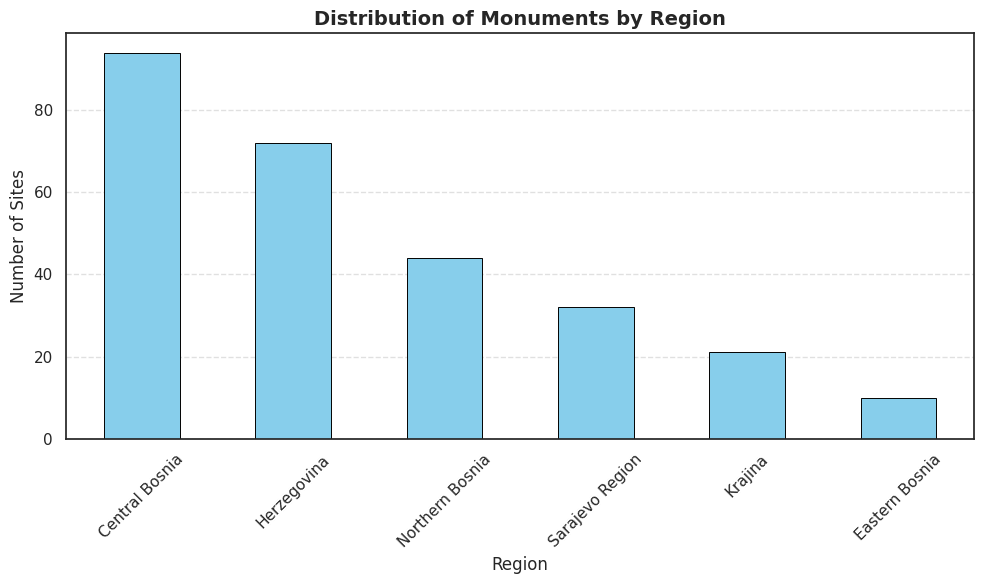
\includegraphics[width=\linewidth]{figures/region_bar.png}
\caption{Number of sites per region.}
\label{fig:region_bar}
\end{figure}

\begin{figure*}[t]
\centering
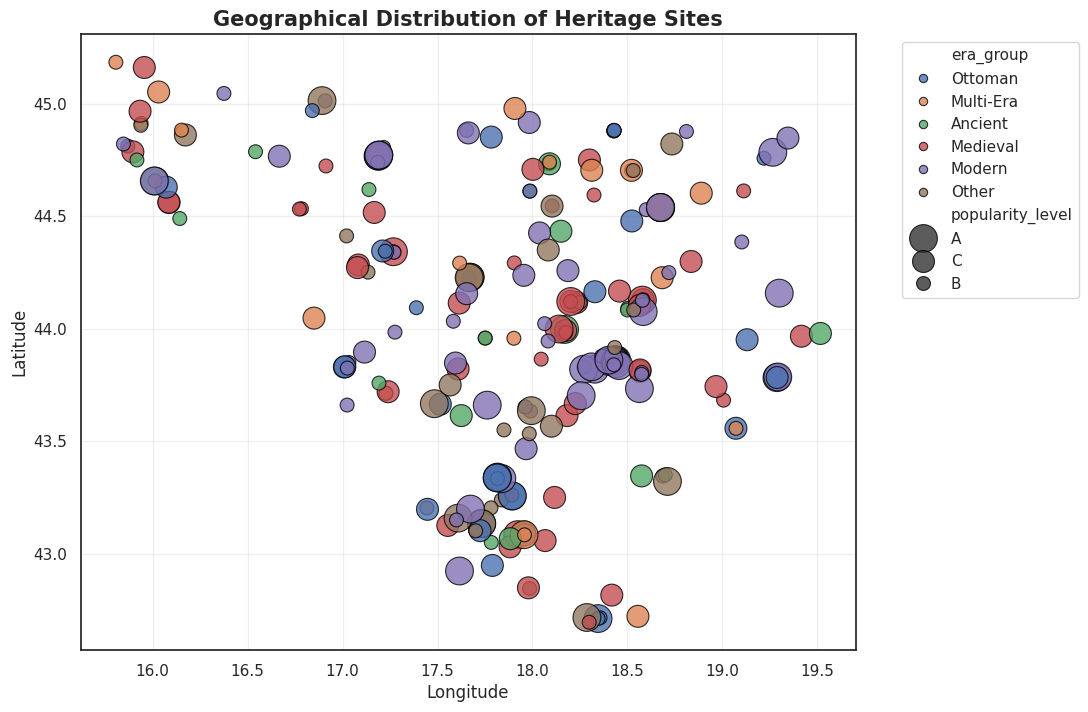
\includegraphics[width=0.85\textwidth]{figures/geo_scatter.png}
\caption{Geographic distribution of all 273 sites.}
\label{fig:geo_scatter}
\end{figure*}

\section{System Design}

\subsection{Overview}
The system operates in three stages, shown in Fig.~\ref{fig:architecture}. A user's question and stated preferences are first matched against the dataset using semantic search; the resulting candidates are then re-ranked using a supervised model based on the user's preferences; and the final short list is passed to a language model, which generates the reply shown to the user.

\begin{figure}[htbp]
\centering
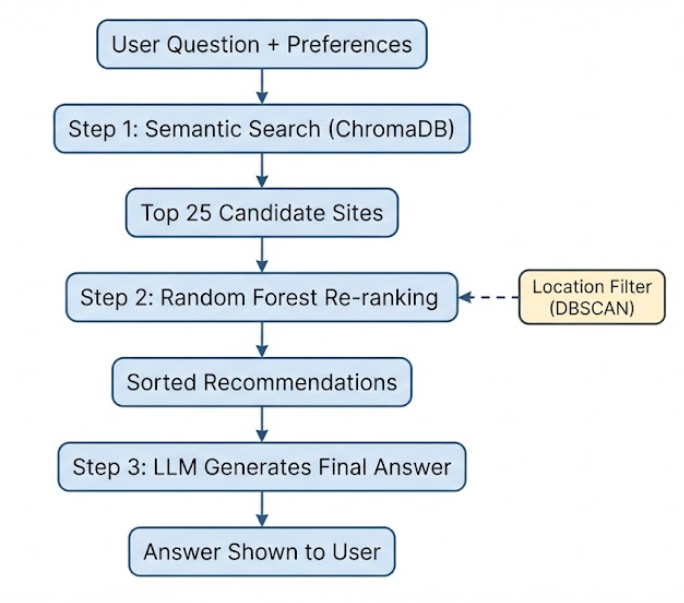
\includegraphics[width=\linewidth]{figures/architecture_diagram.png}
\caption{Overview of the three-stage recommendation pipeline.}
\label{fig:architecture}
\end{figure}

\subsection{Stage 1: Semantic Search}
For each site, the description and keyword fields were combined into a single block of text and converted into a vector using a sentence-embedding model (\texttt{all-MiniLM-L6-v2})~\cite{sbert}. These vectors were stored in a vector database, ChromaDB~\cite{chromadb}. When a user submits a question, it is converted into a vector in the same way, and the database returns the 25 sites whose text is most similar in meaning to the question. This stage is effective at identifying the general topic of a request, but it does not account for the user's stated preferences, such as season or available time, which is addressed in the following stage.

\subsection{Stage 2: Supervised Re-ranking}
The 25 candidates returned by the search stage are re-scored using a Random Forest classifier~\cite{rf}, based on eight inputs: the user's stated interest, the current season, the user's preferred region, whether the user indicated limited time, and the site's region, category, popularity, and historical period. The final ranking score is computed as:
\[
\text{score} = 0.4 \times (\text{search similarity}) + 0.4 \times (\text{model probability}) - 0.2 \times (\text{distance penalty})
\]
The distance penalty is applied only when the user refers to a specific place by name. A Random Forest was chosen over a neural network primarily because the available training data is relatively small (5{,}000 rows with eight simple features), making a simpler, more interpretable model a more appropriate choice at this scale.

\subsection{Stage 3: Grounded Response Generation}
The final stage uses a language model (Groq-hosted \texttt{openai/gpt-oss-120b}) to produce the reply shown to the user. The system prompt explicitly instructs the model not to mention any site, fact, or distance that was not present in the retrieved results. This constraint was introduced after early testing showed that, without it, the model would occasionally produce plausible-sounding but incorrect details, which is not acceptable for a system intended to support real travel decisions.

To prevent self-referential or duplicate recommendations, a two-tiered deduplication pass using a calibrated string similarity threshold ($0.92$) is applied prior to context assembly. This removes alias entries and ensures that spatial corridor lists exclude candidate sites already presented as primary recommendations.

Producing responses that feel conversational, rather than resembling a search form, required additional design work beyond the three core stages. A separate classifier distinguishes ten types of non-travel messages (such as greetings, expressions of thanks, questions about the system's capabilities, and pushback about distance) and routes them to an appropriate short response rather than always returning a list of recommendations. The system also retains relevant information across multiple turns of a conversation; for example, if a user first states an interest and later mentions a different constraint, such as having a bicycle, the previously mentioned location is not discarded.

The application interface exposes some of these settings directly to the user through a sidebar: on the chat page, the user can set their main interest, current season, preferred region, whether they have a limited time budget, and a minimum match confidence threshold, which prevents low-confidence matches from being shown or passed on to the language model; on the map page, a similar sidebar exposes the corridor radius and minimum sites per corridor used by the DBSCAN filtering step described below, along with category and era filters.

\subsection{Location Filtering}
The application also groups sites into approximate geographic corridors using DBSCAN~\cite{dbscan}, configured with the Haversine metric ($\varepsilon = 15\text{ km}$, $\text{min\_samples} = 4$). This density-based clustering method prioritizes nearby sites over distant ones when a user mentions a specific town. This component was originally developed as part of a separate course and was integrated into this project's pipeline rather than developed specifically for it; it is included here for completeness but is not presented as a primary contribution of this work.

\section{Model Training}

\subsection{Simulated Training Data}
No real user interaction data exists for this domain, since the system had not previously been used by real visitors. To address this, 5{,}000 simulated user--site pairings were generated, each representing a hypothetical user profile matched against a site, together with a label indicating whether the pairing was considered a good match. The resulting labels are moderately imbalanced, with 3{,}123 positive examples and 1{,}877 negative examples (approximately 62\% and 38\%, respectively).

\subsection{Model Configuration}
The classifier used is a Random Forest with 200 trees and a maximum depth of 12, trained with \texttt{class\_weight="balanced"} to account for the label imbalance described above, and a fixed random seed to ensure reproducibility. Categorical inputs are converted to numeric form using label encoders, each configured with a fallback ``unknown'' category to handle values not seen during training.

\subsection{Feature Importance}
As shown in Table~\ref{tab:feat_imp} and Fig.~\ref{fig:feat_imp}, the model relies most heavily on whether a site's region matches the user's preferred region, followed by the site's category and historical period. Popularity and available time contribute comparatively little. This suggests that the model is primarily learning to match contextual factors, such as location, type, and era, rather than simply favoring the most popular sites.

\begin{table}[htbp]
\caption{Random Forest Feature Importance}
\label{tab:feat_imp}
\centering
\begin{tabular}{lc}
\toprule
Feature & Importance \\
\midrule
user\_region & 0.175 \\
site\_category & 0.168 \\
period & 0.166 \\
user\_interest & 0.135 \\
current\_season & 0.133 \\
site\_region & 0.110 \\
site\_pop & 0.066 \\
limited\_time & 0.045 \\
\bottomrule
\end{tabular}
\end{table}

\begin{figure}[htbp]
\centering
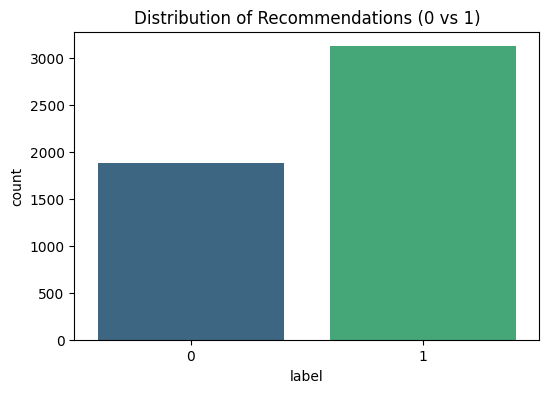
\includegraphics[width=\linewidth]{figures/label_balance.png}
\caption{Balance of positive (good match) and negative (poor match) labels in the simulated training data.}
\label{fig:label_balance}
\end{figure}

\begin{figure}[htbp]
\centering
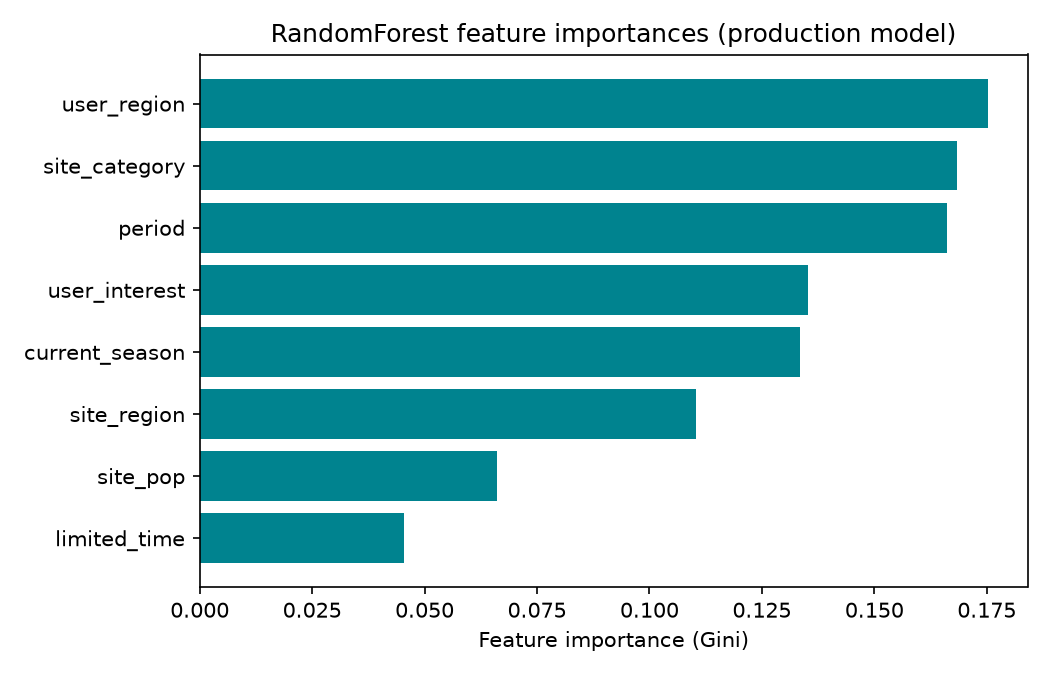
\includegraphics[width=\linewidth]{figures/feature_importance.png}
\caption{Feature importance values for the Random Forest re-ranking model.}
\label{fig:feat_imp}
\end{figure}

\section{Results}

\subsection{Model Accuracy}
Evaluating the model against the same data it was trained on produced an accuracy of 86\%. This figure is misleading, however, since the model had already been exposed to every example in that evaluation set during training. To obtain a fair estimate, the data was split 80/20, with 20\% held out entirely from training, and an identical model was retrained from scratch on the remaining 80\%. This produced a more realistic accuracy of \textbf{74.9\%}, which is reported here as the primary result. Precision and recall on the held-out set were 0.65/0.71 for the negative class and 0.82/0.77 for the positive class, consistent with the class imbalance described earlier.

The difference between the 86\% and 74.9\% figures is itself worth noting, as it illustrates a degree of overfitting: the model performs noticeably better on data it has already seen than on unseen data. This is not entirely unexpected, given that the training data is simulated rather than drawn from real user behavior, and would be an important issue to address before any real-world deployment.

\begin{figure*}[t]
\centering
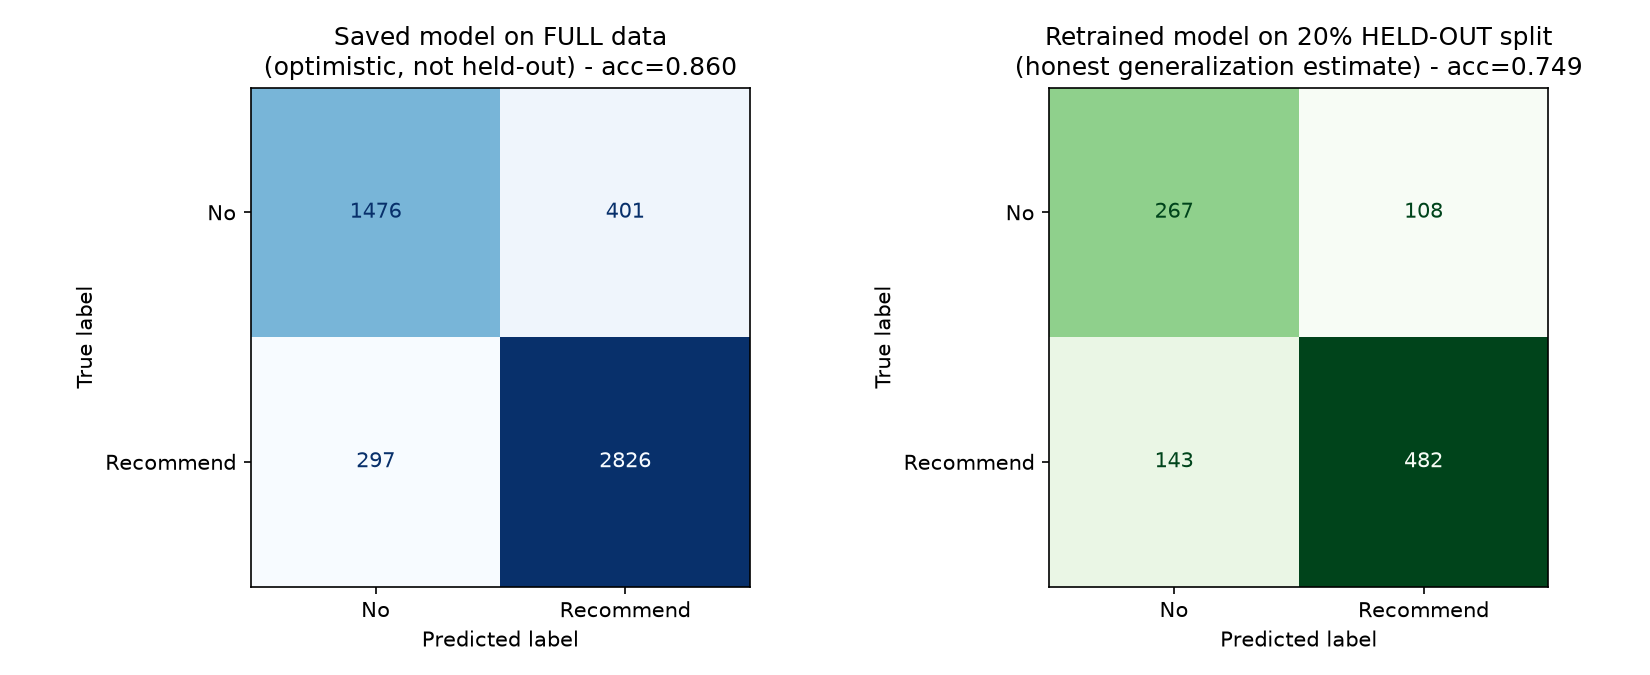
\includegraphics[width=0.85\textwidth]{figures/confusion_matrices.png}
\caption{Confusion matrices for the full training data (left, 86\%) and the held-out 80/20 test split (right, 74.9\%).}
\label{fig:confusion}
\end{figure*}

\subsection{Discussion}
Returning to the first research question posed in the introduction, whether adding a supervised ranking model improves recommendations compared to search alone, the feature importance results suggest that it does: the model is clearly using contextual factors such as region, category, and era to make decisions, rather than defaulting to popularity, which a search-only approach would be unable to do, since it has no direct access to the user's season or time constraints.

\subsection{Scope Not Covered}
A formal evaluation of the chatbot's generated text (for example, a fixed set of sample questions manually scored for relevance) was not carried out as part of this project. This is stated explicitly as a limitation rather than substituted with an informal or unverified claim about response quality.

\section{Application}
KulTur is deployed as a two-page Streamlit web application, shown in Fig.~\ref{fig:chat_ui} and Fig.~\ref{fig:map_ui}. One page provides the conversational chat interface described in Section IV; the other displays an interactive map of the heritage sites grouped by the location corridors described in Section IV-D. An earlier version of the interface was built using Gradio within a Google Colab notebook, which was useful for initial testing but was replaced by the current Streamlit application for the final prototype. API credentials for the language model and mapping services are stored in a separate configuration file excluded from version control, in line with standard practice for handling credentials. The complete source code is available publicly on GitHub~\cite{github}.

\begin{figure}[htbp]
\centering
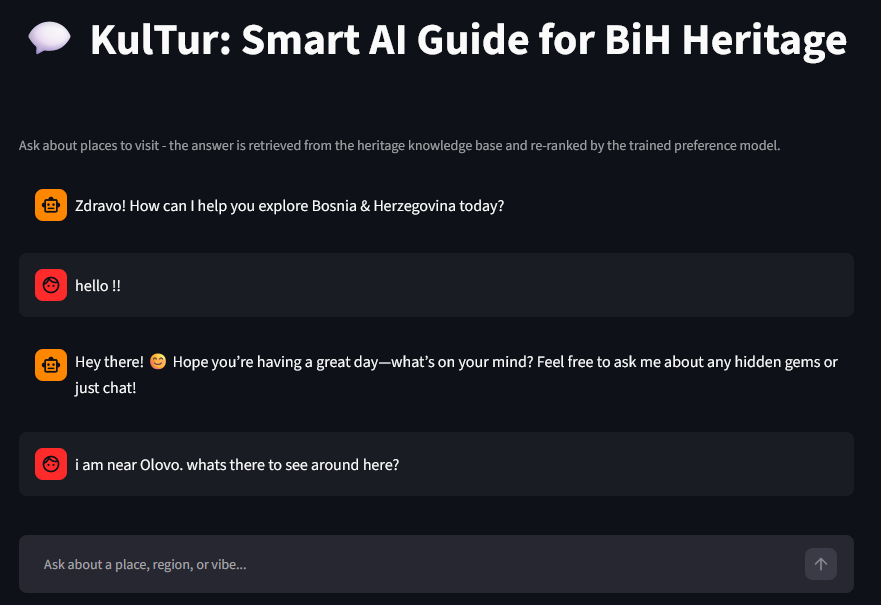
\includegraphics[width=\linewidth]{figures/chat_screenshot.png}
\caption{The KulTur chat interface.}
\label{fig:chat_ui}
\end{figure}

\begin{figure}[htbp]
\centering
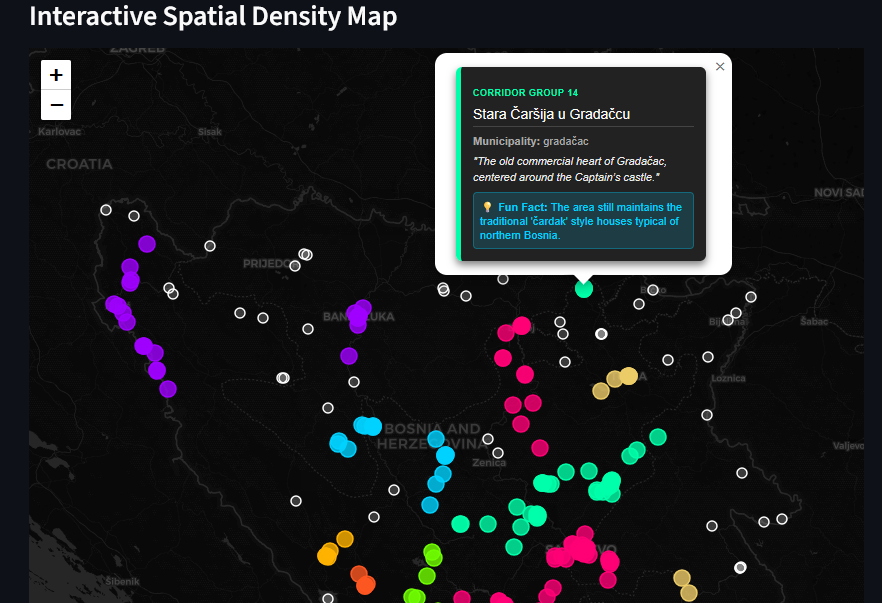
\includegraphics[width=\linewidth]{figures/map_screenshot.png}
\caption{The heritage site map interface.}
\label{fig:map_ui}
\end{figure}

\section{Limitations}
\begin{itemize}
\item The Random Forest model was trained entirely on simulated data rather than real user behavior, so its performance with actual users remains unverified.
\item No formal evaluation of the chatbot's generated responses was carried out.
\item The dataset, while carefully cleaned and verified, was compiled independently rather than sourced from an official government registry, and may not be fully complete or entirely free of minor inaccuracies.
\item The system depends on the availability of a third-party language model API, which is outside the project's control.
\item The embedding model used for search is a general-purpose model rather than one specifically trained on tourism or heritage text, which places an upper bound on retrieval quality.
\end{itemize}

\section{Ethical Considerations}
The dataset used in this project was independently compiled from public and institutional sources rather than an official government registry, and this is stated explicitly rather than implied otherwise. The restriction preventing the language model from introducing information not present in the retrieved data was a deliberate design decision intended to reduce the risk of providing misleading information to users who may rely on the system for actual travel planning. API credentials were also kept out of the project's public source code repository, in keeping with standard security practice.

\section{Commercialization Potential}
The overall approach, combining search, supervised re-ranking, and grounded response generation, is not inherently specific to Bosnia and Herzegovina. The same architecture could in principle be applied to other regions by substituting the underlying dataset and retraining the ranking model accordingly. Integration with booking or ticketing platforms could also represent a plausible avenue for future monetization, although this was not implemented as part of the current project.

\section{Conclusion}
This project developed KulTur, a chatbot that recommends heritage sites in Bosnia and Herzegovina based on user preferences while remaining strictly limited to verified information. The most demanding aspect of the project was the construction and cleaning of the underlying dataset, rather than the machine learning components. A Random Forest re-ranking model was trained and honestly evaluated, achieving 74.9\% accuracy on unseen data, and a complete working prototype was built around the resulting pipeline. Future work would involve collecting real user interaction data to retrain the ranking model and constructing a formal evaluation set to assess the quality of the chatbot's generated responses.

\begin{thebibliography}{99}
\bibitem{rf} L. Breiman, ``Random forests,'' \textit{Machine Learning}, vol. 45, no. 1, pp. 5--32, 2001.
\bibitem{rag} P. Lewis et al., ``Retrieval-augmented generation for knowledge-intensive NLP tasks,'' in \textit{Advances in Neural Information Processing Systems (NeurIPS)}, 2020.
\bibitem{sbert} N. Reimers and I. Gurevych, ``Sentence-BERT: Sentence embeddings using Siamese BERT-networks,'' in \textit{Proc. EMNLP}, 2019.
\bibitem{dbscan} M. Ester, H.-P. Kriegel, J. Sander, and X. Xu, ``A density-based algorithm for discovering clusters in large spatial databases with noise,'' in \textit{Proc. 2nd Int. Conf. Knowledge Discovery and Data Mining (KDD)}, 1996.
\bibitem{chromadb} Chroma, ``Chroma: The AI-native open-source embedding database,'' \url{https://www.trychroma.com/}, accessed 2026.
\bibitem{streamlit} Streamlit Inc., ``Streamlit documentation,'' \url{https://docs.streamlit.io/}, accessed 2026.
\bibitem{fzs} Federal Institute for Statistics of Bosnia and Herzegovina, \url{https://fzs.ba/}, accessed 2026.
\bibitem{kons} Commission to Preserve National Monuments of Bosnia and Herzegovina, \url{http://www.kons.gov.ba/}, accessed 2026.
\bibitem{unesco} UNESCO World Heritage Centre, \url{https://whc.unesco.org/}, accessed 2026.
\bibitem{spomenik} Spomenik Database, \url{https://www.spomenikdatabase.org/}, accessed 2026.
\bibitem{kaggle} Bosnia and Herzegovina Heritage Landmarks Dataset, Kaggle, \url{https://www.kaggle.com/datasets/danakopi/bosnia-and-herzegovina-heritage-landmarks-dataset}, accessed 2026.
\bibitem{github} KulTur source code repository, GitHub, \url{https://github.com/dzankk/BiH_cultural_tourism_chatbot}, accessed 2026.
\end{thebibliography}

\end{document}